\anglais
\doublespacing
\chapter{Understanding where networks stop}\label{supp:boundaries}
\begin{refsection}

\section{Why boundaries are interesting}

As discussed in both Chapters~\ref{Perspectives} and \ref{SpatialBoundaries}
there is value in thinking about the existence of boundaries between networks, either from a prediction perspective (\emph{e.g.,} knowing at what scale to make predictions at) or from a more theoretical question of where do networks stop? Although this is discussed in more detail in \autoref{Defining-ecotrophic-zones} there is one question regarding network boundaries that might be a good starting point and that is looking at how environmental and network boundaries relate, more specifically do environmental changes drive changes in networks. Here I present what is more of a methodological framework (as opposed to an actual answer, hence why it has been relegated as an Appendix) that we can use to try and answer this question.

\section{A metacommunity model for boundary detection}

The metacommunity model developed by \cite{Thompson2017Dispersal} is a good starting point to use for this 'case study' as it allows us some flexibility with how we want to parameterise the system. The model (\ref{eq:metacomm_full}) itself is based on a tritrophic community ('plants', 'herbivores', and 'carnivores') and is a collection of modified Lotka–Volterra equations and (broadly) models species abundance as a function of interaction strength, environmental effect, immigration, and emigration. The metacommunity consists of $S$ species with $M$ environmental patches and looks as follows:

\begin{equation} \label{eq:metacomm_full}
X_{ij}(t+1)=X_{ij}(t)exp\left[C_{i} + \sum_{k=1}^{S}B_{ik}X_{kj}(t)+A_{ij}(t)\right]+I_{ij}(t)-X_{ij}(t)a_{i}
\end{equation}

Where $X_{ij}(t)$ is the abundance of species $i$ in patch $j$ at time $t$. $C_i$
is its intrinsic rate of increase (which we have set to 0.1 for 'plants' and
-0.01 for 'herbivores' and 'carnivores'). $B_{ik}$ is the per capita effect of
species $k$ on species $i$. The exact interaction strength for each species pair
is drawn from a uniform distribution with the parameters for the 
interaction pairs listed in \autoref{table:interaction_strength}, the values
drawn from the uniform distribution are scaled by dividing by $0.33S$ to yield
the final interaction strength for each interacting pair.

\begin{table}[h!]
\centering
\begin{tabular}{||c c||} 
 \hline
Interacting pair & Range of uniform distribution \\ [0.5ex] \hline\hline
 Plant-plant & -1 -- 0 \\ 
 Plant-herbivore & 0 -- 0.1 \\
 Plant-carnivore & 0 \\
 Herbivore-plant & -0.3 -- 0 \\
 Herbivore-herbivore & -0.2-- -0.15 \\
 Herbivore-carnivore & 0 -- 0.08 \\
 Carnivore-plant & 0  \\
 Carnivore-herbivore & -0.1 -- 0  \\
 Carnivore-carnivore & -0.2-- -0.15 \\ [1ex] 
 \hline
\end{tabular}
\caption{Intervals used for the uniform distribution from which interaction
strengths values are drawn from for the different types of species pair
interactions. Note this is represent the effect of species type 1 on species
type 2 \emph{i.e.,} herbivore-plant represents the effect of a herbivore species on a plant species}
\label{table:interaction_strength}
\end{table}

$A_{ij}(t)$ is the effect of the environment in patch $j$ on species $i$ at time $t$ and can be further expanded as follows:  

\begin{equation} \label{eq:metacomm_env}
A_{ij}(t)=h\left(exp-\frac{(E_{j}(t)-H_{i})^2}{2\sigma^2}-1\right)
\end{equation}

Species environmental optima ($H_i$) are evenly distributed across the entire range of environmental conditions for each trophic level, meaning that species from different trophic levels will be at, or near the same environmental optima. $h$ is a scaling parameter (set to 300), $E_j(t)$ is the environment in patch $j$ at time $t$ and $\sigma$ is the standard deviation (set to 50).

$I_{ij}(t) $is the abundance of species $i$ immigrating to patch $j$ at time $t$
and can be expanded as follows:

\begin{equation} \label{eq:metacomm_imm}
I_{ij}(t)=\sum_{l=j}^{M}a_iX_{il}(t)exp(-Ld_{jl})
\end{equation}

Where $ai$ is the proportion of the population of species $i$ that disperses at each time step, the dispersal rate is drawn from a normal distribution ($\mu$ = 0.1, $\sigma$ = 0.025) for each species. The abundance of immigrants to patch $j$ from all other patches is governed by where $d_{jl}$ is the geographic distance between patches $j$ and $l$, and $L$ (the strength of the exponential decrease in dispersal with distance), which is also drawn from a normal distribution for each species. The parameters used for $L$ are trophic level dependant and are show in \autoref{table:interaction_decay}

\begin{table}[h!]
\centering
\begin{tabular}{||c c c||} 
 \hline
Trophic level & $\mu$ & $\sigma$ \\ [0.5ex] \hline\hline
 Plant & 0.3 & 0.075 \\ 
 Herbivore & 0.2 & 0.05 \\
 Carnivore & 0.1 & 0.025 \\ [1ex] 
 \hline
\end{tabular}
\caption{Parameters for the normal distributions used to determine the dispersal
decay ($L$) for each species depending on its trophic level.}
\label{table:interaction_decay}
\end{table}

\section{A toy example of boundary detection}

The associated code for these simulations was carried out in \texttt{Julia 1.8} (\cite{Bezanson2017Julia}) using \texttt{Makie.jl} (\cite{Danisch2021Makie}) and \texttt{SimpleSDMLayers} (\cite{Dansereau2021Simplesdmlayers}), this can be found in a GitHub repo \href{https://github.com/PoisotLab/Omnomnomivores}{\texttt{here}}. Note that the results presented here are supposed to represent a hypothetical result and it is not so much that there is ecological knowledge to be gleaned from the figure below but rather to showcase how we can approach the idea of boundary detection across landscapes. For the initial modelling exercise presented below I have used 80 species ($S$ = 80) within a 20 by 20 landscape (\emph{i.e.,} $M$ = 400). This landscape is generated using \texttt{NeutralLandscapes.jl} (\cite{2023Neutral}), which allows the user to specify different landscape types \emph{e.g.,} one with a clear boundary, the landscape values are used to represent the environmental value for the specific patch.

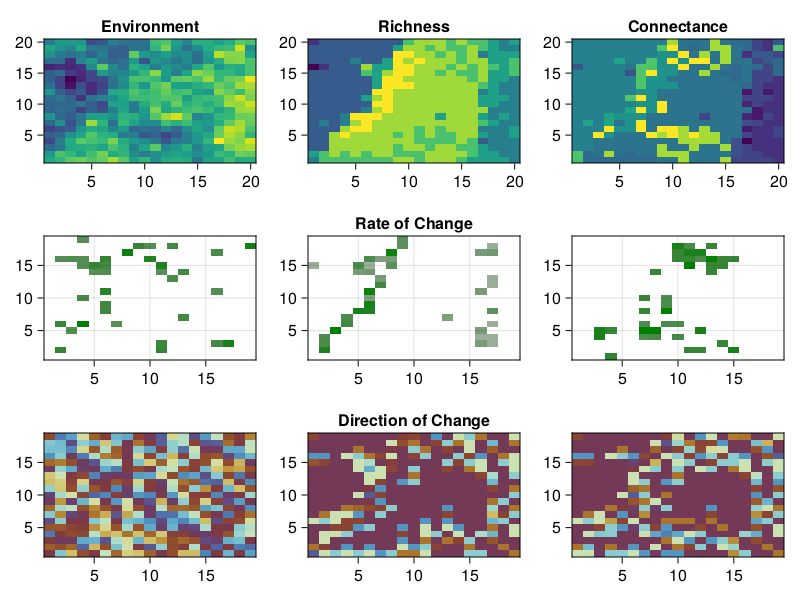
\includegraphics[width=\textwidth]{./figures/heatmaps.png}

The top row represents the 'raw' values for the landscape after 500 generations. Note here I have included species richness as it might be interesting to see if species richness is related to network structure, in this instance I have used connectance as that measure of network structure since it is one of the more common network metrics to use. 

The second row show the rates of change for the respective metrics, but only limited to the top 90\% rate of change values for a cleaner visual. Here the colour intensity indicates the magnitude of the rate of change. The final row is showing the direction of change for the respective metrics and each colour can be thought of as indicating a cardinal point.

What is interesting about this simulation is that the rate of change for environmental, species richness, and connectance do not 'line-up' and that the species community and the way they interact are responding differently to changes in the environment - although the direction of change seems quite similar for species richness and connectance. This is also interesting since it might suggest that although the exact 'location' of changes might be different the way the change is propagated across the landscape is the same. Overall I would argue that there is evidence that indicates that the idea of 'ecotrophic boundaries' is one worth exploring further.

\printbibliography{}
\end{refsection}

\endinput